\section{Introduction}
3D printing enables the fabrication of complex geometry under few design constraints compared to conventional fabrication techniques.
Recent developments have seen a rapid growth in both the use and capabilities of desktop 3D printing systems.
%The rapid spread of 3D printing through different industries and types of application calls for the possibility to manufacture a wide range of geometries while guaranteeing mechanical properties of the resulting parts.
Fused Deposition Modeling (FDM) is one of the most common 3D printing techniques.
It is widely used because of the versatility in the types of plastics which can be used and the relatively low running costs.
FDM printers are used, for example, in showcasing scale models of buildings, casings for electronics, prototypes for blow molded parts, jigs and fixtures.
Recent research developments have investigated manufacturing complex volumetric structures such as microstructures~\cite{bates2018compressive,Al-Ketan2018,Maskery2018} and topology optimized structures~\cite{Zegard2016SMO,Wu2019a,Cheng2019}.
Many of these applications involve 3D models with detailed features within the order of magnitude of the printing resolution, which restrains the field of the process planning algorithms.

FDM printers extrude semi-continuous beads of molten plastic through a nozzle, which moves along a planned toolpath within each layer of a 3D object.
A common strategy to accurately manufacture a given 3D model is to extrude along a contour-following path,
because the position and shape of the toolpath can be controlled relatively accurately.
Filling up a shape using parallel straight lines would expose defects of the size of the nozzle, which is generally an order of magnitude larger than the resolution of the positioning system.
Contour-parallel extrusion therefore leads to a less bumpy outline shape than direction parallel extrusion does.


The simple technique for generating the dense contour-parallel toolpaths of a layer consists in performing uniform inward offsets with the radius of the nozzle from the outline shape.
However, for geometrical features which are not an exact multiple of the nozzle size this method produces areas where an extrusion bead is placed twice: \emph{overfill} areas; and areas which are not filled at all: \emph{underfill} areas.
See \cref{intro_wedge}(top).
Overfills cause a buildup of pressure in the mechanical extrusion system, which can result in bulges or even a full print failure.
Underfills on the other hand, can cause a drastic decrease in the part stiffness or even for small features not to be printed at all.
These problems are exacerbated for models with layer outlines with small features, because the over- and underfill areas are relatively large compared to the whole part.

One promising direction to avoid over- and underfills is to employ toolpath with adaptive width. 
This strategy has been mostly investigated for metal additive manufacturing using wire and arc~\cite{Ding2014,Xiong2019}, where it has been shown that a wide range of widths could be realized by the hardware. 
For instance, \citeauthor{Ding2016a} developed a toolpath with an (estimated) width variation by a factor of up to $3$~\cite{Ding2016a}.
However, for FDM printing, it is challenging to accurately realize varying width by extruding material through a nozzle with a fixed size, either by varying the movement speed or by dynamically adjusting the volumetric flow rate. 
Therefore, a much narrower range of widths is desirable for robust FDM fabrication.
On the other hand, controlling the variation in width is beneficial for limiting the variation in mechanical properties of the resulting material fragments. 
% The bead width has been associated with total print time, the roughness of top surfaces, printing resolution and the strength of a part, through the contact area it makes with neighboring beads~\cite{N.Turner2014,ahn2002anisotropic}.

In this paper we propose a framework for planning toolpath with adaptive width for minimizing over- and underfill. 
We show that this framework supports multiple schemes on deciding the bead locations and extrusion widths. 
In particular for FDM printing, we propose a novel scheme which reduces the amount of over- and underfill while ensuring a small deviation of extrusion widths from the nozzle size (\cref{intro_wedge} bottom). 
% In order to avoid over- and underfills in regions which are not as wide as an exact multiple of the nozzle size we need algorithms which produce toolpaths which employ adaptive bead width.
% Some such toolpath generation techniques have already been developed.

\begin{figure}\centering
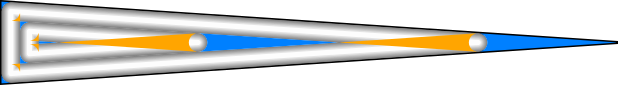
\includegraphics[width=\columnwidth]{sources-intro-TEST-naive-accuracy.png}
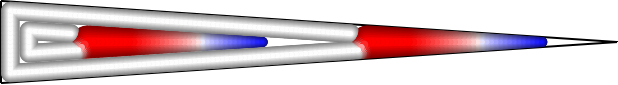
\includegraphics[width=\columnwidth]{sources-intro-TEST-Center-widths.png}
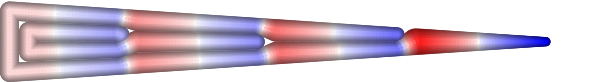
\includegraphics[width=\columnwidth]{sources-intro-TEST-InwardDistributed-widths.png}
\caption{
Illustration of different toolpath for a wedge shape.
Top: Toolpath using uniform offsetting results in large overfill (orange) and underfill (azure).
Middle: Toolpath with adaptive width~\cite{Jin2017JMS} where beads that are wider or narrower than the nozzle size are indicatd in red and blue, respectively.
Bottom: Our approach minimizes over- and underfill with beads close to the nozzle size.
}
\label{intro_wedge}
\end{figure}



% There is a large body of literature on relating process parameters such as bead width to various mechanical properties of the end part.
% The bead width has been associated with total print time, the roughness of top surfaces, printing resolution and the strength of a part, through the contact area it makes with neighboring beads~\cite{N.Turner2014,ahn2002anisotropic}.
% In order to accurately fabricate a part restricted to prescribed mechanical properties, we need to generate toolpaths using the corresponding process parameters as close as possible.
% We therefore develop a framework which can be used to generate toolpaths which not only avoid over- and underfill, but also keep the bead width closer to the preferred bead width compared to existing techniques.
% See \cref{intro_wedge}(bottom).

%\subsection{Contributions}
% A polygonal shape with a width of a fractional multiple of the preferred bead width will always result in the bead widths deviating from the preferred bead width by the fractional part in total,
% because the total of the widths of the beads must add up to the fractional width of the part in order to avoid under- or overfill.
% We therefore propose a framework which makes it possible to distribute the fractional discrepancy over several beads, so that the beads are generally closer to the preferred width.
Our contributions are as follows:
\begin{itemize}
\item A geometric framework for generating densely filling contour-parallel toolpaths employing adaptive width, according to any beading scheme which maps a feature diameter to a number of beads and their widths.
\item A specific beading scheme for FDM printing which reduces the amount of beads with greatly deviating width, and which promotes smooth toolpaths that are close to the preferred width toward the outline of the shape.
% \begin{itemize}
% \item Accurately filling a 2D outline with extrusion beads
% \item Reducing the overfill and underfill areas compared to the uniform width technique
% \item Reducing the amount of beads with greatly deviating width compared to existing literature
% \item Promoting smooth toolpaths which are close to the preferred width toward the outline of the shape.
% \end{itemize}
\end{itemize}



%This work is patent pending, but the source code is available open source.

